% Chapter Template

\chapter{Projects/Activities} % Main chapter title
%σύντομη περιγραφή όλων των δραστηριοτήτων που ανέλαβα

\label{Chapter3}

During my internship, I participated in quite a few projects that were mostly related to Beat Hotels product, either bugs resolved or entirely new features created, or Greek Marketing’s requirements. All of these projects will be analyzed in this chapter, expect the ones of Chapter \ref{Chapter4} that will just mentioned so as to avoid repetition.

\section{Project 1: Price Estimator- Rides for Approval}

BeatHotel is a totally different product than Beat and a newly introduced one as described in the previous Chapters. For this reason, this new product is combined with a different driver app and a dashboard used by agents, Beat's employees. Agents use the dashboard in order to control rides made through BeatHotel App, start a ride or cancel one if it is needed. This new product does not have any price estimator for the rides made which means that a driver could theoretically add any amount desirable. \par

The project “price estimator” was created for preventing any fraud occurred by drivers. The aim of this project was to estimate the price of a completed ride and compare this price with the actually declared one. In this way, every completed ride is checked  and if it does not pass the validation, it remains as Ride for Approval, so as Agents to check the validate of price gained. \par

This project was the first project ever assigned to me and to one more intern. Our role to this project was to create in Node.js a function for calculating the price of a completed ride based on the data found in database and another function for validating if the result is approximately equal to the ride's price. We need to mention that every five seconds, each driver sends its location (latitude and longitude), a timestamp (time of the data sent) and other information. So, we used these data gathered in firebase and by using the geo package mentioned later on and rules of how taxi pricing is in Greece, we managed to get an estimation of the ride. Afterwards, we created one more function for checking the real price with the estimated one. \par

The project lasted about two weeks and it was a great addition to BeatHotel HQ service. We need to clarify that for about a year the service did not have any commissions gained from the driver and that's why it was not a priority at first. Because of this additional feature, Beat's commission is real scenario. \par 


\section{Project 2: Geo - Npm Package}

This project occurred during the implantation of "Price Estimator". In more detail, this is referred to the creation of an npm package as described in Appendix 8.3, showing the project's ReadME.md file. The package can be used in both front and back-end applications, and it returns one function called getDistance. \par 

\begin{wrapfigure}[11]{r}{0.3\textwidth}
	\begin{center}
		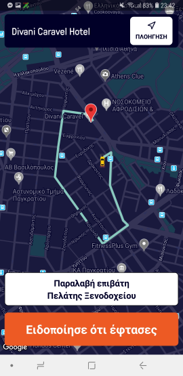
\includegraphics[scale=0.25]{images/my_projects/price_estimator.png}
	\end{center}
	\caption{Price Estimator}
\end{wrapfigure}

As regards the returned function, it receives one argument, which is an object with timestamps as keys and properties information sent from a gps device, such as longitude, latitude and accuracy of the gps. The object needs to include at least two subobjects with timestamps as keys and as its properties one longitude and one more latitude. The purpose of this function is to return a number that reveals how many kilometers have been traveled based on the given object. \par

For privacy reasons, it is not possible to cite the code written. However, it can be mentioned that code was developed in ES6 JavaScript, consists of 75 lines of code, both comments and pure code, and it includes three functions in total. Moreover, there were created unit tests in Jest that are 87 lines examining twelve different use cases. Code is using enlist-styling and includes babel in its webpack configuration so as to be used in both front-end and back end projects if it is needed. \par

The project lasted about four days and it was the first npm package I ever created. The most complicated and challenging fact was the integration with babel in order package to run in both client and server side. \par 

\begin{figure}[H]
	\begin{center}
		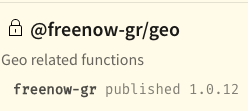
\includegraphics[scale=0.85]{images/my_projects/geo_npm-package.png}
	\end{center}
	\caption{Geo npm package on Npm}
\end{figure}

\section{Project 3: Statistics (analyzed in next Chapter)}

"Statistics" project is an external feature in Agent's dashboard that reveals total rides and Gross Merchandise Volume (GMV) gained from BeatHotel service. This project was separated in three main parts, the creation of stats npm package, customized statistics and general statistics, that will be described in detail in next Chapter. Generally, there were added charts in the BeatHotel's web application that present data based on different parameters chosen by Agents. In the chart, the given period's data are also compared with the previous week's or year's data and useful information are extracted for BeatHotel service.

\section{Project 4: Geofence in New Map}

There was a need for changing maps in "Live Map" Tab of BeatHotel HQ dashboard since the ones firstly displayed were not that responsive. Thus, the first front-end task ever assigned to me was to include the presented in figure 3.2 polygons to the new adapted map. \par

The project lasted about one day and its result is visible to Agents. Polygons are showing the area in which if a taxi driver assigned to BeatHotel service enter, he/she gets a number in a queue were the first one gets a ride. \par 

\begin{figure}[H]
	\begin{center}
		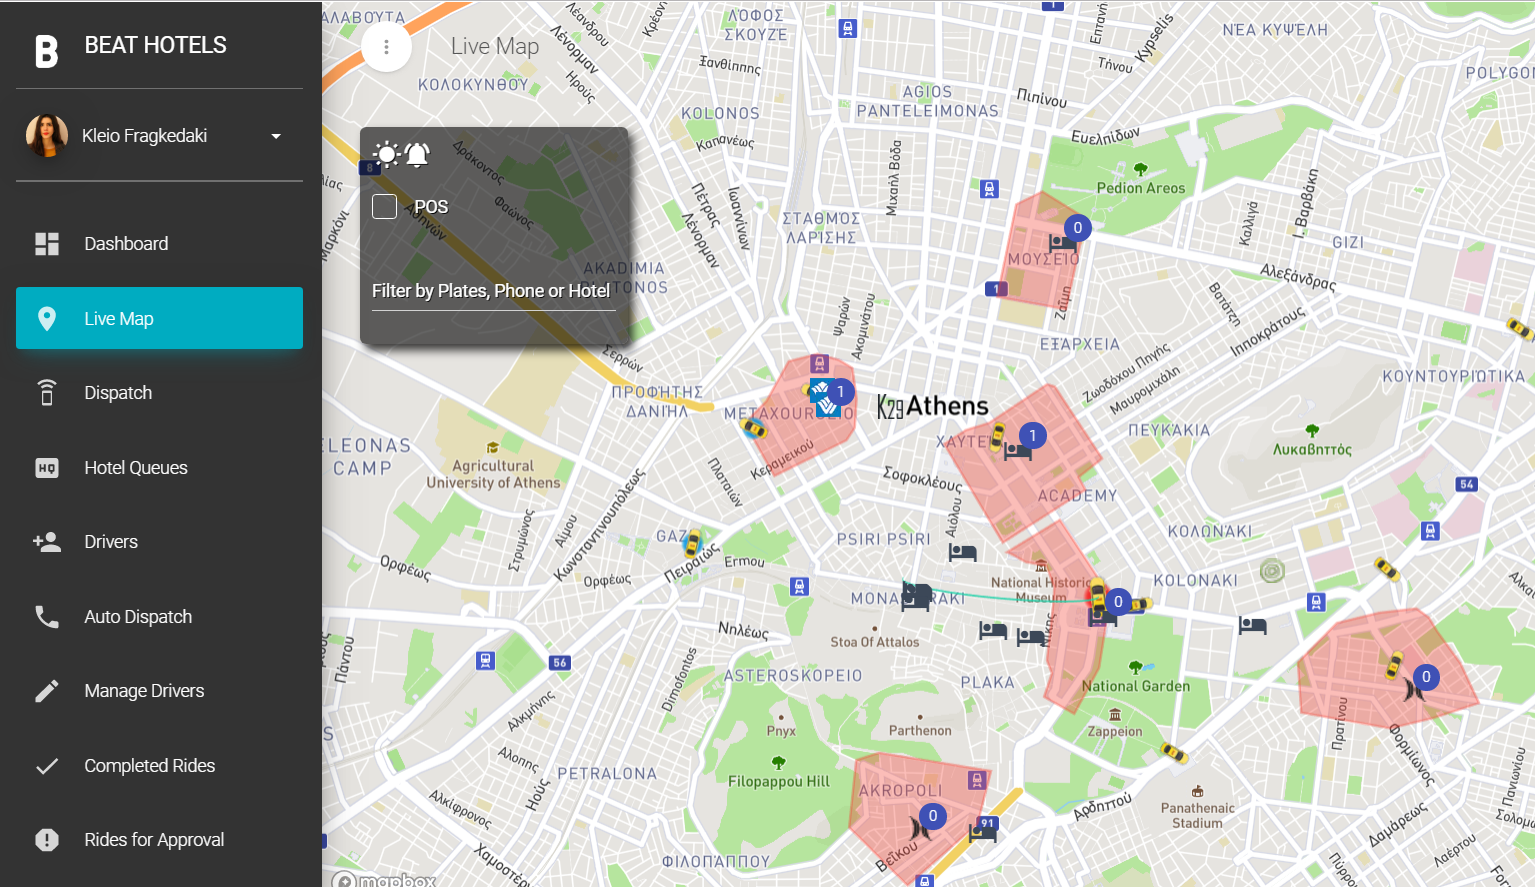
\includegraphics[scale=0.45]{images/my_projects/new_map.png}
	\end{center}
	\caption{Geofence and arc added into new map}
\end{figure}

\section{Project 5: Arc for accepted Drivers in Map}

The next project assigned to me was also a front-end task. In this task, it was required an arch to be added in "Live Map" Tab from any driving vehicle having accepted a call to his/her pickup location, as figure 3.2 reveals.\par

This project lasted less than one day, my PR was merged on May 28 where the change of map's were implemented. The arc is now visible to agents and it consists a useful feature because of reporting driver's direction to a hotel and agents are aware of which driver is about to fulfill which request. \par

\begin{figure}[H]
	\begin{center}
		
\includegraphics[scale=0.85]{images/my_projects/feature-add-arc-to-arcs-PR.png}
	\end{center}
	\caption{Geofence and arc added into new map- PR on GitHub}
\end{figure}

\section{Project 6: Add Start/End-timestamp \& HQ link}

In Agent's BeatHotel HQ dashboard, there is a tab named "Completed Rides" which includes all the finished rides created via BeatHotel service and ordered by their creation date. If one of those rides is clicked then a pop-up like the following ones is displayed. For performance reasons, it was requested the addition of the ride's ended and started time in the window where agents see more information about a ride, and also when clicking on the Driver's Plates, his/her profile on HQ to be appeared. HQ is a dashboard that includes every detail of both Beat's passengers and drivers. In the following picture, it is visible the previous and the new version of the pop-up referred. In the new version, the three red arrows are showing the features included by me and are referred to this project. \par

\begin{figure}[H]
	\centering
	\subfloat[Old Version]{{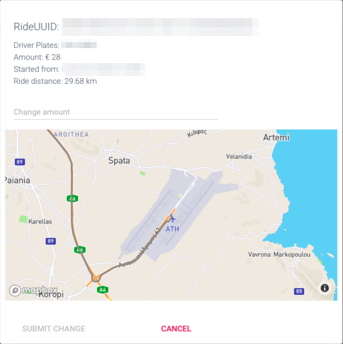
\includegraphics[scale=0.55]{images/my_projects/feature-add-timestamp-linkToHQ-old.png} }}%
	\qquad
	\subfloat[New Version]{{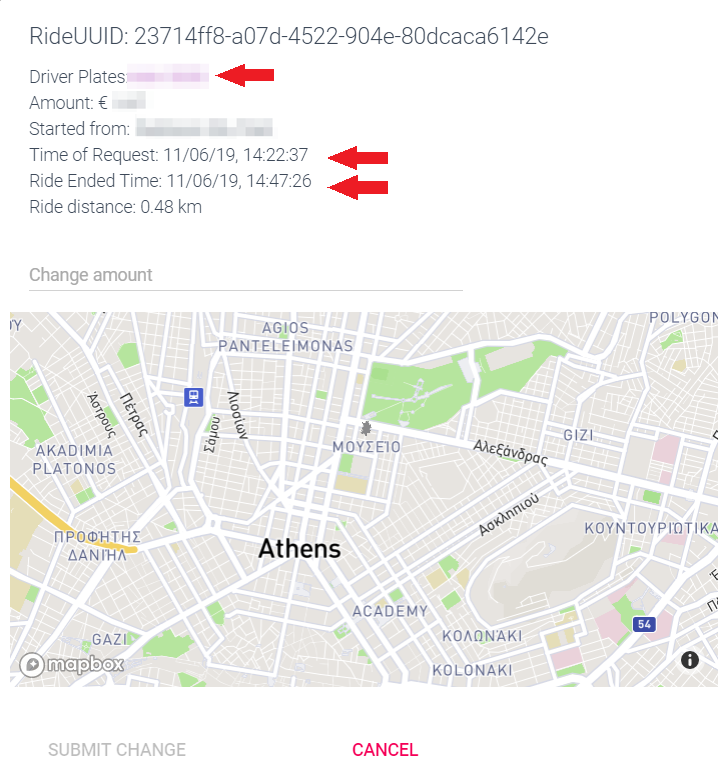
\includegraphics[scale=0.25]{images/my_projects/feature-add-timestamp-linkToHQ-new-plus-map.png} }}%
	\caption{
		Added to Completed Rides timestamps and link driver to HQ
	}
	\label{fig:example}
\end{figure}

This project's duration was about 2 days and my PR, as shown bellow, was merged on May 15. This feature is visible to BeatHotel HQ and is providing data for a ride that are needed to the agents. \par

\begin{figure}[H]
	\begin{center}
		
\includegraphics[scale=0.85]{images/my_projects/feature-add-timestamp-linkToHQ-PR.png}
	\end{center}
	\caption{Added timestamps and links to HQ- PR on GitHub}
\end{figure}


\section{Project 7: Errors and bugs occurred in BeatHotel HQ service}

During my internship, I was assigned to resolve some errors or bugs occurred in BeatHotel HQ service. Following, most of them are explained. \par

Firstly, there were some errors in console generated by either material-ui or eslint. The PR I created for resolving these errors was merged on May 24.

\begin{figure}[H]
	\begin{center}
		
\includegraphics[scale=0.85]{images/my_projects/fix-eliminate-errors-PR.png}
	\end{center}
	\caption{Eliminate errors in console and eslint errors- PR on GitHub}
\end{figure}

Another issue was that map's token was included in every component map was used. For security and re-usability reasons, I changed its place to the config folder in a file named mapboxToken, and imported this to every component that used the token. The PR created for changing credentials was merged on May 24.

\begin{figure}[H]
	\begin{center}
		
\includegraphics[scale=0.85]{images/my_projects/fix-change-credentials-PR.png}
	\end{center}
	\caption{Change place of map's token- PR on GitHub}
\end{figure}

An issue occurred when "Rides for approval" tab added. This tab was similar to the one named as "Completed Rides", but with the difference that this includes the rides which did not pass the check validation of "Price Estimator" described earlier. Thus, the pop-up, which displays selected ride's information and has the new feature of section "Add Start/End-timestamp \& HQ link", redirected to wrong urls. After examining, all four possible ways to dispatch a taxi, the problem solved and its PR merged.

\begin{figure}[H]
	\begin{center}
		
\includegraphics[scale=0.85]{images/my_projects/fix-doesnot-redirect-to-HQ-PR.png}
	\end{center}
	\caption{Error in HQ link on "Approved Rides" tab- PR on GitHub}
\end{figure}

\section{Project 8: Add button for unblocking dispatching status-production}

An issue related to firebase callable functions leads to driver's status blocking. When this happening, agents need to change driver's status to off-line, fact that it was not previously possible through dashboard and a variety of e-mail were sent to the development team. For this reason, I created a new column with a button in "Manage Driver" tab that gives to agents this ability.

\begin{figure}[H]
	\begin{center}
		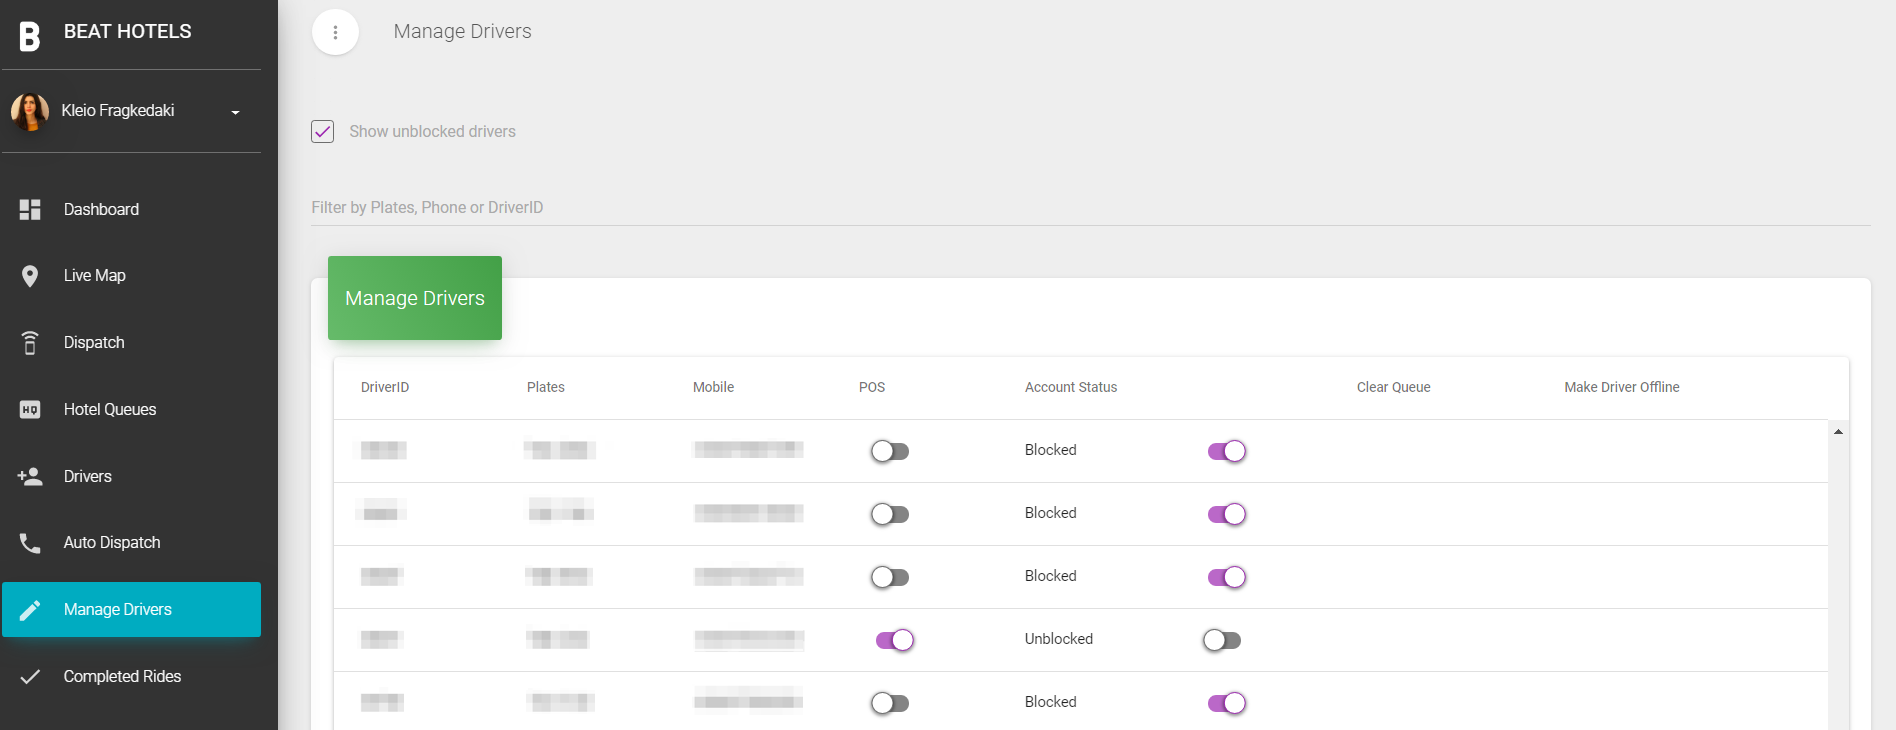
\includegraphics[scale=0.2]{images/my_projects/feature-add-add-button.png}
	\end{center}
	\caption{Button for unblocking dispatching status}
\end{figure}

There were added 66 pure lines of code and deleted 11 lines, while 3 files were changed. The PR was merged on May 22 and it is currently available to agents.

\begin{figure}[H]
	\begin{center}
		
\includegraphics[scale=0.85]{images/my_projects/feature-add-add-button-PR.png}
	\end{center}
	\caption{Add button for unblocking dispatching status- PR on GitHub}
\end{figure}

\section{Project 9: Landing page for mpaineis-vgaineis (analyzed in next Chapter)}

Landing page for mpaineis-vgaineis is a project referred to the development of a web site for \url{mpaineis-vgaineis.gr} competition of Beat. More specifically, GR Marketing team launched an event in which every week one participant would win a trip abroad. The competition lasted four weeks, and every week there was a different destination. My part to this event was to create the landing page through which every possible user could declare interest in the event, and in this way, to win a trip in one of the destinations. So, I created a responsive to all devices web page, that includes a form for users to declare their interest. The landing page will be online until 7th of June. \par

\section{Project 11: Input location (analyzed in next Chapter)}

BeatHotel is generally a B2B service that aims to fulfill the needs of hotels for a virtual taxi queue. So, the service's dashboards, which is the only way Beat's Agents and Hotels to request for a taxi, used for calling a cub to only one pick-up location, the requested Hotel. However, as the business grows, travel agencies, that were part of the system as well, and some hotels needed to fulfill rides that are having different than Hotel's pick up locations. For this reason, this project occurred and I needed to refactor the Dispatch page, change modal so as to be responsive and add an input for typing any possible different pick-up location. \par

\section{Project 12: Zoom to hotel and driver}

In the tab named "Live Map" of Agent's BeatHotel HQ dashboard, it is displayed a map in which every hotel and driver that uses BeatHotel service is shown to this in real time. By typing a driver's plates or phone, agents can filter cars presented on the map and only the ones matching with filters are appeared. However, when it is searched one specific car, there is difficulties to locate it in the map. So, a new feature added that zooms to driver  if there is a unique driver that is matching with the given tables and phone. After the implementation of this features, it was also requested to filter and zoom in Hotels based on their name. \par

\begin{figure}[H]
	\centering\subfloat[Zoom to Hotel]{{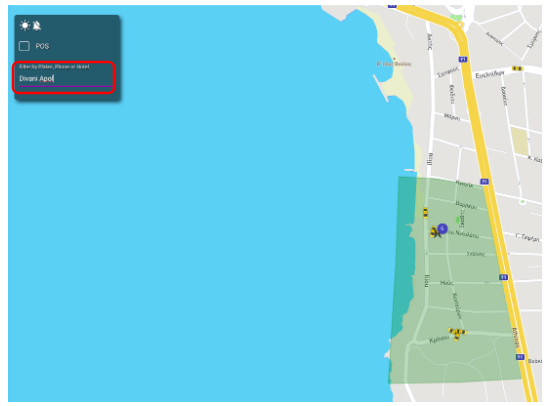
\includegraphics[scale=0.3]{images/my_projects/zoom-to-hotel.png} }}
	\qquad\subfloat[Zoom to Driver]{{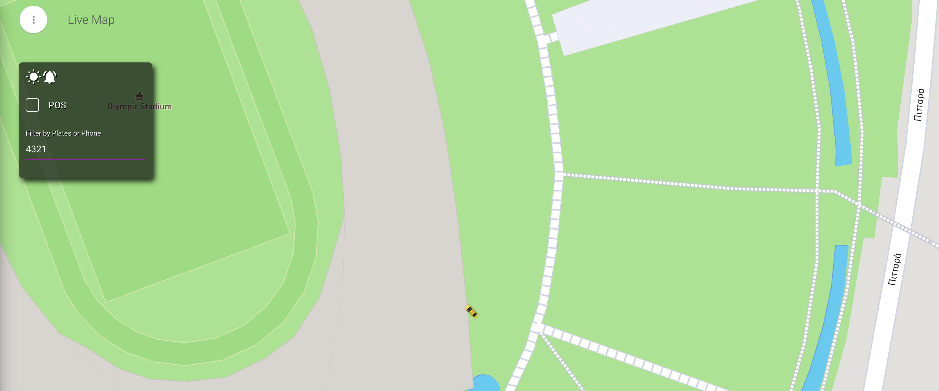
\includegraphics[scale=0.22]{images/my_projects/zoom-to-driver-after.png} }} 
	\space%
	\qquad{{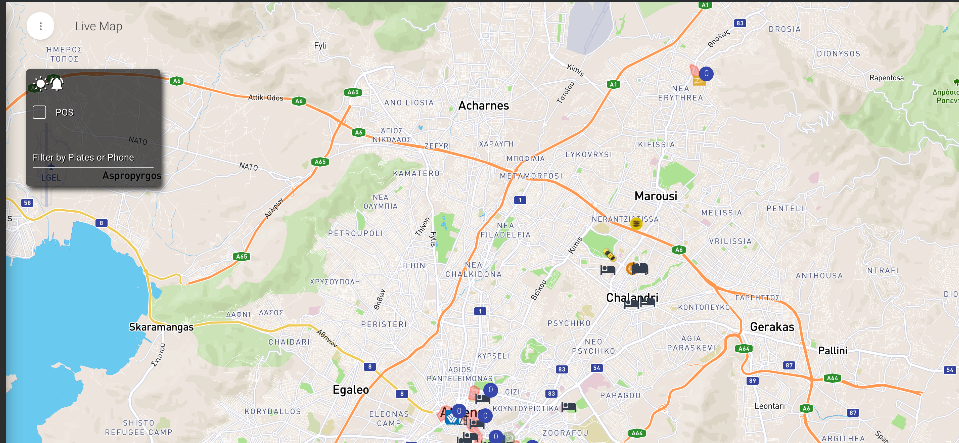
\includegraphics[scale=0.3]{images/my_projects/zoom-to-driver-before.png} }}%
	\caption{
		Zoom either to hotel or driver depending on the filter displayed
	}
	\label{fig:example}
\end{figure}

There were displayed two different PR's for the previously explained features. As regards the feature for zooming to driver, there were added 44 pure lines of code and removed 11 lines, and two files changed in total. On the other hand, for zooming to hotel 84 lined added and 25 removed, while 7 files were modified. Both PR were merged and features are currently used from agents. \par

\begin{figure}[H]
	\centering
	\subfloat[Zoom to Driver]{{
\includegraphics[scale=0.85]{images/my_projects/zoom-to-driver-PR.png} }}%
	\qquad
	\subfloat[Zoom to Hotel]{{
\includegraphics[scale=0.85]{images/my_projects/zoom-to-hotel-PR.png} }}%
	\caption{
		Pull requests on GitHub
	}
\end{figure}


\section{Project 13: Restructure Setting Component}

Setting components contains 396 lines of code which cannot be reused. The challenge was to restructure and eliminated lines of code in this component so as smaller and reusable components to be created. For this purpose, the SettingInput component, representing the three yellow squares, was generated, and the DashboardKPIContainer, representing the red ones, was modified so as to apply in this case as well and not only in Dashboard's cards. \par

\begin{figure}[H]
	\begin{center}
		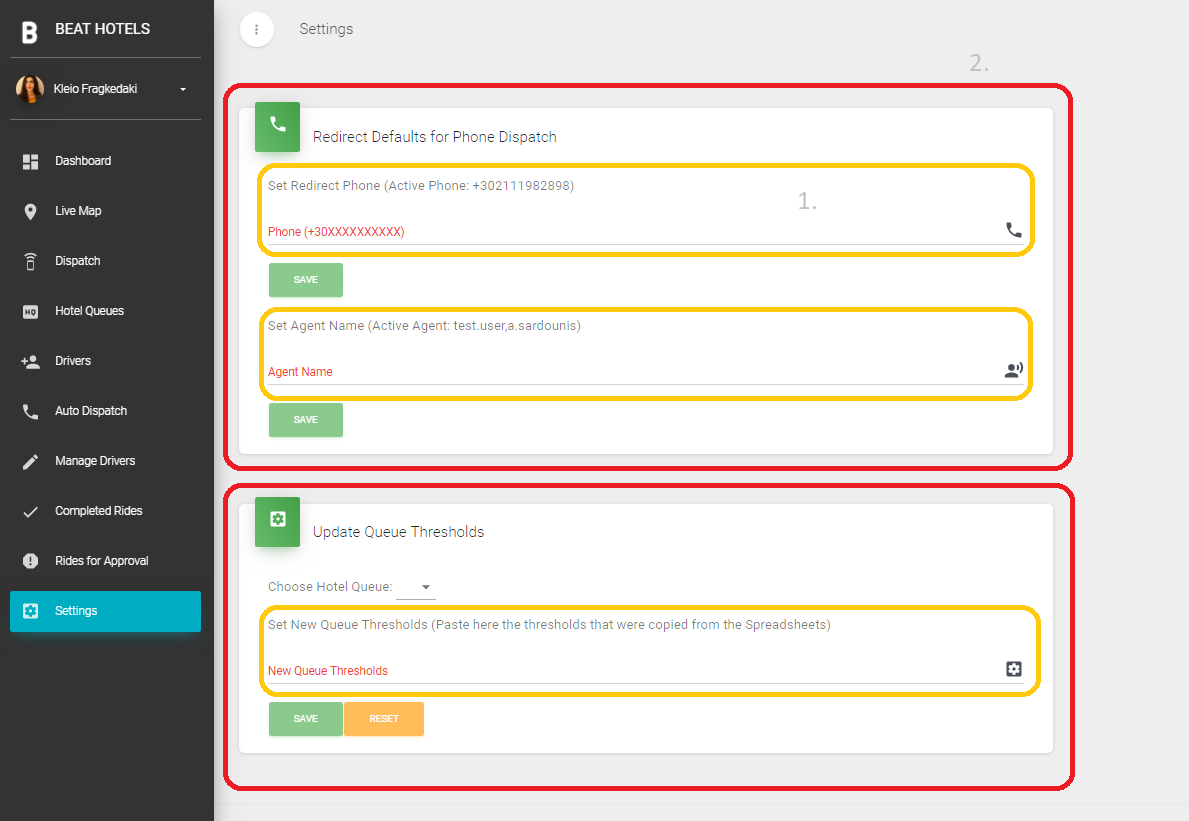
\includegraphics[scale=0.45]{images/my_projects/fix-restructure-setting-component.png}
	\end{center}
	\caption{How Setting Component was restructured in small reusable components}
\end{figure}

The PR created was merged and it includes 242 added lines, 209 deleted ones and 4 modified files. \par

\begin{figure}[H]
	\begin{center}
		
\includegraphics[scale=0.85]{images/my_projects/fix-restructure-setting-component-PR.png}
	\end{center}
	\caption{Restructure Setting Component- PR on GitHub}
\end{figure}

\section{Project 14: Replace old maps}

After replacing the map in "Live Map" tab, I was requested to also replace the maps shown in a selected ride's information pop-up of "Completed Rides" and "Rides for Approval". The maps were displaying the whole root of a finished ride. 

The PR was merged and it's result is shown in figure 3.5 (B) represented in Project 6.

\begin{figure}[H]
	\begin{center}
		
\includegraphics[scale=0.85]{images/my_projects/feature-replace-old-maps-PR.png}
	\end{center}
	\caption{Replace old maps- PR on GitHub}
\end{figure}
